%"###############################################
%
% Classification RTUPB post 
%
%###############################################

En utilisant PAM sur les données post-opératoires, la courbe des silhouettes moyennes
nous indique une valeur maximale pour un nombre de classes à k = 2.

\begin{figure}[H]
\centering
\includegraphics[width=0.90\textwidth]{../Fig/RTUPB/rtupb-silpam-post.png}
\caption{Maximisation de la silhouette moyenne }
\end{figure}

Cependant, si nous regardons le détail des classes et de leurs silhouette pour k = 2,
nous avons une première classe incluant la quasi totalité des patients dont 2 dont le profil est éloigné (valeurs de silhouette négatives), et une deuxième classe ne contenant que trois patients (11, 28 et 33)
avec une valeur de silhouette à 1, indiquant des données répliquées exactement et donc une classe triviale.
Après vérification que ces patients ont des données post-opératoires identiques, mais ne sont pas pour autant
des doublons (données pré-opératoires différentes), nous poursuivons la recherche du maximum suivant qui se trouve à k = 3.

\begin{figure}[H]
\centering
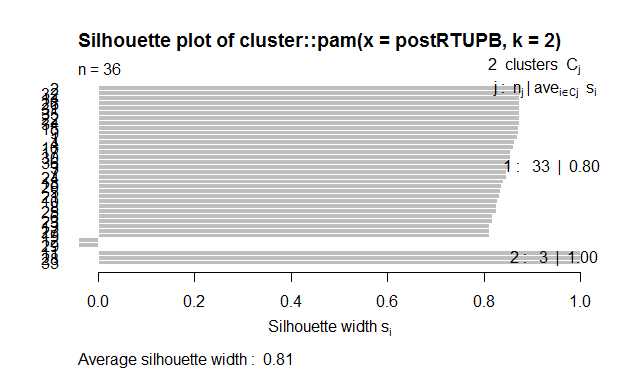
\includegraphics[width=0.75\textwidth]{../Fig/RTUPB/rtupb-sil-k2-post.png}
\caption{Silhouette / classe (k = 2) }
\end{figure}



\begin{figure}[H]
\centering
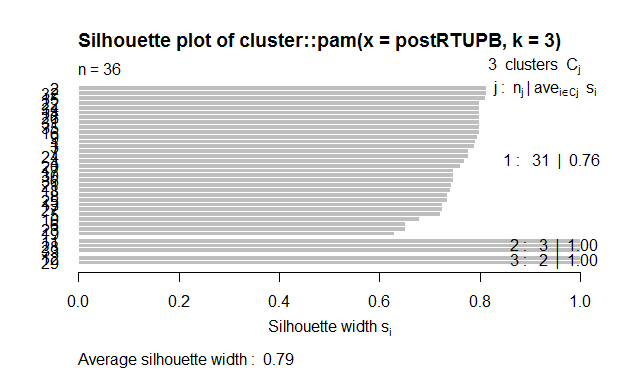
\includegraphics[width=0.75\textwidth]{../Fig/RTUPB/rtupb-sil-k3-post.png}
\caption{Silhouette / classe (k = 3)}
\end{figure}

\begin{figure}[H]
\centering
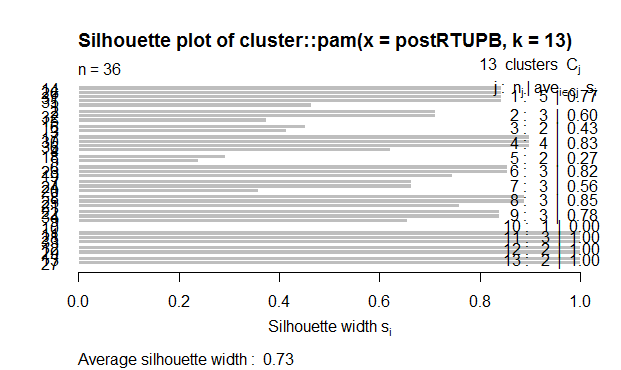
\includegraphics[width=0.75\textwidth]{../Fig/RTUPB/rtupb-sil-k13-post.png}
\caption{Silhouette / classe (k = 13)}
\end{figure}




%
%##########################
%# CONCLUSION
%##########################